%------------------------------------------------------------------------------------------------
The figure to the right shows a crane whose cab \basis{A} supports a boom \basis{B} that swings
a wrecking ball $C_o$.
%
Sets of \dextral ~orthogonal unit vectors (\uvecxyz{n}), (\uvecxyz{b}), and (\uvecxyz{c})
are defined as shown.
%
\\[0.5pc] The position vector from $N_o$ to $C_o$ is
$\posvec{N_o}{C_o} \equals[\;] x~\uvecx{n} \plus[\;] L_B ~\uvecx{b} \minus[\;] L_C ~\uvecy{c}$.
%
\\[0.0pc]
\begin{minipage}{0.52\textwidth}
%\\[0.5pc]
%The angular velocity of \basis{B} in \basis{N} is
%$\angvel{B}{N} \equals[\;] \thetadot_B ~\uvecz{b}$.
%\\[0.25pc] The angular velocity of \basis{C} in \basis{N} is
%$\angvel{C}{N} \equals[\;] \thetadot_C ~\uvecz{c}$.

{\small
\vspace{0.5pc}
\begin{tabular}{|l|c|c|}
          \hline Quantity                                                   & Symbol     & Type
\\[0.0pc] \hline \uvecx{b} distance between $A_B$ and $B_C$      & $L_B$ & Constant
\\[0.0pc]        \uvecy{c} distance between $B_C$ and $C_o$      & $L_C$ & Constant
\\[0.0pc] \hline \uvecx{n} distance between $N_o$ to $A_B$       & $x$ & Variable
\\[0.0pc]        angle between \uvecx{n} and \uvecx{b} about \uvecz{n}      & $\theta_B$ & Variable
\\[0.0pc]        angle between \uvecy{n} and \uvecy{c} about \uvecz{n}      & $\theta_C$ & Variable
  \\[0.0pc]\hline
\end{tabular}}

\end{minipage}
\hfill
\begin{minipage}{0.4\textwidth}
\flushright
\vspace{-1.0pc}
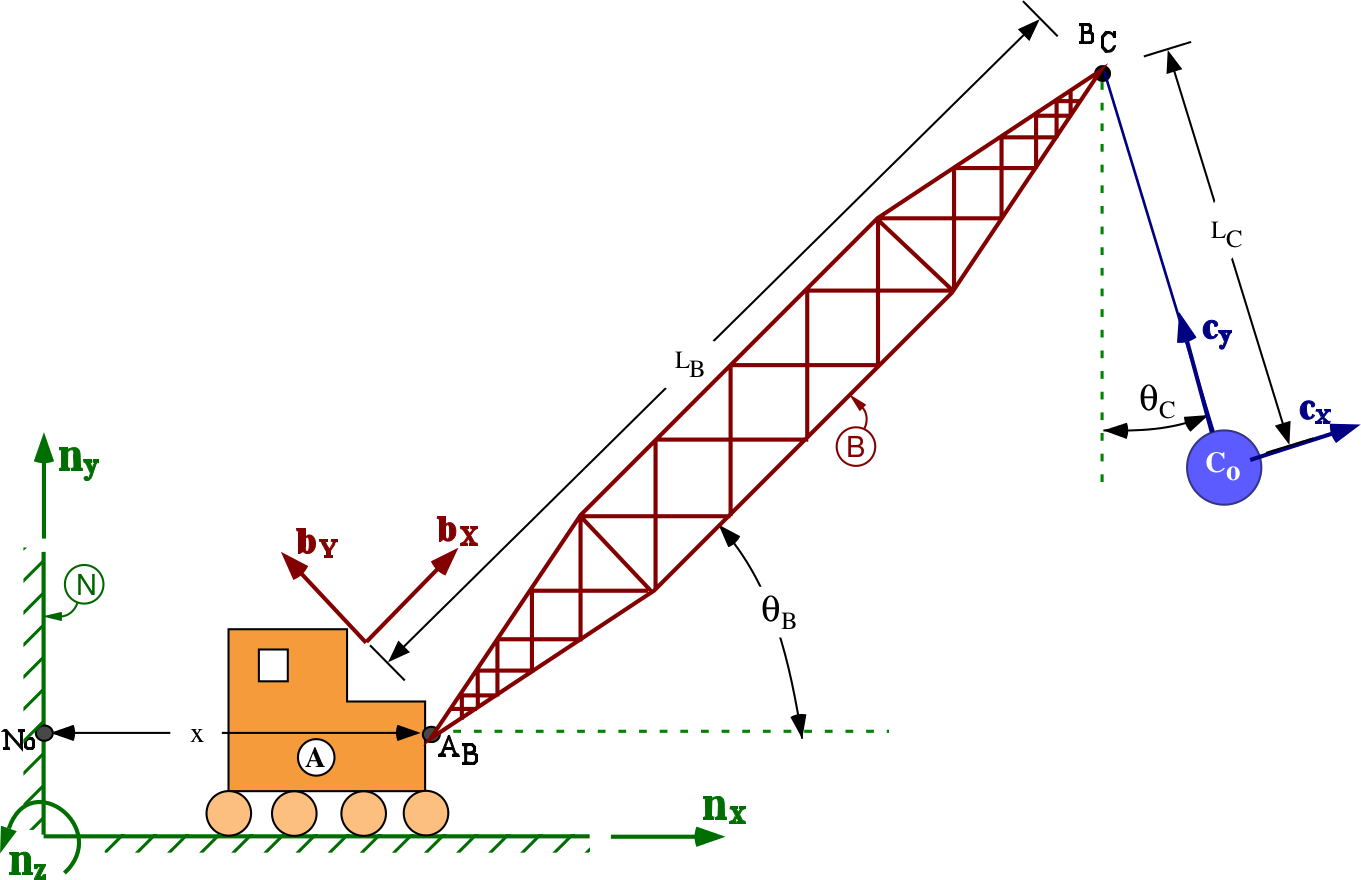
\includegraphics[width=0.99\textwidth]{crane_transparent.png}
\end{minipage}
\\[0.0pc]
%
\begin{enumerate}
\item .
\\[-1.0pc]
\begin{tabular}{@{}ll}
Determine:  & the angular velocity of \basis{B} in \basis{N} (or, \basis{B}'s angular velocity in \basis{N}). \\[0.0pc]
& the angular velocity of \basis{C} in \basis{N} (or, \basis{C}'s angular velocity in \basis{N}) \\[0.0pc]
& the angular velocity of \basis{C} in \basis{B} (or, \basis{C}'s angular velocity in \basis{B}).
\end{tabular}
\\[0.0pc]
\Solution{
\\[0.0pc]
  The first two are ``simple'' rotations (see section 7.3.3), so angular velocity is formed \textbf{by inspection}.
  For example, imagine $\theta_B$ is zero, and align your (right-hand!) fingers with \uvecx{b}=\uvecx{n}. Then curl your fingers in the direction of increasing $\theta_B$. Your thumb gives the direction vector associated with \angvel{B}{N}.
  \\[0.5pc]
\begin{tabular}{ll}
  $\angvel{B}{N} \equals[\;] \thetadot_B ~\uvecz{n}$
  &
  \hspace{1cm}$\angvel{C}{N} \equals[\;] \thetadot_C ~\uvecz{n}$
\end{tabular}
  \\[0.5pc]
  For \angvel{C}{B} it is easiest to use the angular velocity addition theorem (see section 7.3.4 - 7.3.5).
  \\[0.55pc]
  \begin{tabular}{l}
  $\angvel{C}{B} \equals[\;] \angvel{N}{B} + \angvel{C}{N}
                 \equals[\;] (-\thetadot_B + \thetadot_C) ~\uvecz{n}$
  \end{tabular}
  \\[0.0pc]
}{
  \vspace{4.0pc}
}
%
\item Compute the velocity of $C_o$ in \basis{N} in terms of symbols in the table
and their time derivatives.
\\[0.5pc]
%
\begin{tabular}{@{}lcl}
$\vel{C_o}{N}$ & $\deff$ & \Solution{\dt[N]{}$~\posvec{N_o}{C_o}
\equals[\;]  \dt[N]{}(x~\uvecx{n} \plus[\;] L_B ~\uvecx{b} \minus[\;] L_C ~\uvecy{c})$}{}
\end{tabular}
\Solution{
\\[0.5pc]
We distribute first to get separate chunks to which we can then apply the golden rule:
\\[0.5pc]
\hspace*{0.7cm}
\begin{tabular}{@{}lc c@{}c@{}c@{}c@{}c}
& \equals[\;] &
$\dt[N]{}(x~\uvecx{n})$ & $\plus[\;]$ & $\dt[N]{}(L_B ~\uvecx{b})$ & $\minus[\;]$ & $\dt[N]{}(L_C ~\uvecy{c})$
\\[0.5pc]
& \equals[\;] &
$\dt[N]{}(x~\uvecx{n})$ &
$\plus[\;]$ & $[~\dt[B]{}(L_B ~\uvecx{b}) + \angvel{B}{N} \times (L_B ~\uvecx{b}) ~]$ &
$\minus[\;]$ & $[~\dt[C]{}(L_C ~\uvecy{c}) + \angvel{C}{N} \times (L_C ~\uvecy{c})~]$
\\[0.5pc]
& \equals[\;] &
$\dt[N]{}(x~\uvecx{n})$ &
$\plus[\;]$ & $[~\dt[B]{}(L_B ~\uvecx{b}) + (\thetadot_B ~\uvecz{n}) \times (L_B ~\uvecx{b}) ~]$ &
$\minus[\;]$ & $[~\dt[C]{}(L_C ~\uvecy{c}) + (\thetadot_C ~\uvecz{n}) \times (L_C ~\uvecy{c})~]$
\\[0.5pc]
& \equals[\;] &
$\xdot~\uvecx{n}$ &
$\plus[\;]$ & $[~0 + L_B \thetadot_B (\uvecy{b})~]$ &
$\minus[\;]$ & $[~0 + L_C \thetadot_C (-\uvecx{c})~]$
\\[0.5pc]
& \equals[\;] &
$\xdot~\uvecx{n}$ &
$\plus[\;]$ & $L_B \thetadot_B \uvecy{b}$ &
$\plus[\;]$ & $L_C \thetadot_C \uvecx{c}$
\end{tabular}
\\[0.5pc]
Take a moment to mentally visualize the movement of $C_o$ caused by each ``degree-of-freedom" in the system (each variable), and check that the terms of \vel{C_o}{N} seem to describe that motion.
\\[0.5pc]
One way to check your work is to verify that the units on every term are the same. It's a velocity, so each term must have the units of length per time. In SI units, the first term is $\frac{m}{s}$ and the second and third terms are $m*\frac{rad}{s}$, which is equivalent to $\frac{m}{s}$ since radians are ``unit-less".
}{
\\[11.0pc]
}
%
\Solution{\clearpage}{\vfill}
\item Compute the acceleration of $C_o$ in \basis{N}.
%(It is probably easiest to just differentiate your result from (a),
%but
\\[0.0pc]If it helps, you can use the fact that $\accel{Bc}{N} = \ddot{x}~\uvecx{n} + L_B \thetaddot_B ~\uvecy{b} - L_B \thetadot_B^2 ~\uvecx{b}$.
% and observe that $B_C$ and $C_o$ are both fixed in \basis{C}.)
%\\[0.5pc] $\accel{C_o}{N} \equals[\;]$
%\\[11.0pc]
\Solution{
\\[1.0pc]
This can be computed using the definition (that is, differentiating \vel{C_o}{N} found above).
\\[0.0pc]Please TRY IT this way, and verify that you get the same result as what I show here:
%
\\[0.5pc]For this solution, I will show a different way. When two points are \textbf{fixed} on a rigid body/frame, it is possible to relate the velocity and acceleration of those two points using a pair of formulas (see ``how to calculate acceleration" on page 45).
%
\\[0.5pc]First, convince yourself that $B_C$ and $C_o$ are both \textbf{fixed} in frame \basis{C}.
Since I provided $B_C$'s acceleration in \basis{N}, you can relate it to $C_o$'s acceleration in \basis{N} as follows (verify that you understand how the general formula on page 45 was adapted to the specific frames and points in \textbf{this} problem).
\\[0.5pc]
$\accel{C_o}{N} = \accel{B_c}{N} \plus[\;] \alf{C}{N} \times \posvec{B_C}{C_o} \plus[\;] \angvel{C}{N} \times (\angvel{C}{N} \times \posvec{B_C}{C_o})$
\\[0.5pc]
Looks like we need \alf{C}{N} (see section 7.4), defined as
$\alf{C}{N} ~\deff~ \dt[N]{}\angvel{C}{N}$, so we get $\alf{C}{N} \equals[\;] \thetaddot_C ~\uvecz{n}$ (try it).
\\[0.5pc]
The first term (\accel{B_c}{N}) was given.
\\[0.5pc]
The second term is:
\\[0.5pc]
\begin{tabular}{l}
$\alf{C}{N} \times \posvec{B_C}{C_o} \equals[\;]  \thetaddot_C ~\uvecz{n} \times (-L_C \uvecy{c})$
$\equals[\;]  L_C \thetaddot_C ~\uvecx{c}$
\end{tabular}
\\[0.5pc]
The third term is:
\\[0.5pc]
\begin{tabular}{l@{$\equals[\;]$}l}
$\angvel{C}{N} \times (\angvel{C}{N} \times \posvec{B_C}{C_o})$ &
$\thetadot_C ~\uvecz{n} \times (\thetadot_C ~\uvecz{n} \times (-L_C \uvecy{c}))$
\\[0.5pc]
 & $\thetadot_C ~\uvecz{n} \times (L_C \thetadot_C ~\uvecx{c})$
\\[0.5pc]
 & $L_C (\thetadot_C)^2 ~\uvecy{c}$
\end{tabular}
\\[0.5pc]
Putting all the pieces together we have:
\\[0.5pc]
$\accel{C_o}{N} = \ddot{x}~\uvecx{n} \plus[\;] L_B \thetaddot_B ~\uvecy{b} \minus[\;] L_B \thetadot_B^2 ~\uvecx{b} \plus[\;] L_C \thetaddot_C ~\uvecx{c} \plus[\;] L_C (\thetadot_C)^2 ~\uvecy{c}$
\\[1.0pc]
To check our work, we should first check that the units on every term the same. Vectors (like anything) must have the same units in order to add them together, so this is an easy way to check your work.
\begin{itemize}
\item $\xddot = \dt{}(\dt{}x)$ has units of ((length/time)/time). In SI units, that would be $m/s^2$.
\item $L_B$ and $L_C$ are both lengths (m), and $\thetaddot_B$ and $\thetaddot_C$ are both the second derivative of an angle ($\mathrm{rad}/s^2$).
Radians are a stand-in for ``no units'', so $L_B \thetaddot_B$ and $L_C \thetaddot_C$ both have units of $m/s^2$.
\item Since the units on $\thetadot_B$ and $\thetadot_C$ are first derivatives of an angle (rad/s),
the units on $L_B (\thetadot_B)^2$ and $L_C (\thetadot_C)^2$ are both $m/s^2$.
\end{itemize}
\vspace{0.5pc}
Finally, let's look at the terms and see if they make sense when looking at the picture (see section 8.5).
\begin{itemize}
\item The first term says that changes in $x$ cause $C_o$ to accelerate in the \uvecx{n} direction. That makes sense.
\item The second term says there is an acceleration ``tangent'' to the rotation described by $\theta_B$.
%That is, it is caused by $\alf{B}{N}$, or the second-derivative of $\theta_B$.
\item The third term is due to the first-derivative of $\theta_B$ (i.e. due to \basis{B}'s angular velocity in \basis{N}). Notice that it acts ``inward" toward the source of the rotation; this is a ``centripetal'' component.
\item The fourth term says there is an acceleration ``tangent'' to the rotation described by $\theta_C$.
%That is, it is caused by $\alf{C}{N}$, or the second-derivative of $\theta_C$.
\item The fifth term is due to the first-derivative of $\theta_C$ (i.e. due to \basis{C}'s angular velocity in \basis{N}). Notice that it acts ``inward" toward the source of the rotation; this is another ``centripetal'' component.
\end{itemize}
}{
}
\end{enumerate}
